% DO NOT COMPILE THIS FILE DIRECTLY!
% This is included by the other .tex files.

\begin{frame}[t,plain]
\titlepage
\end{frame}

\begin{frame}
    \frametitle{Who am I}
    \begin{minipage}{0.6\textwidth}
        \begin{itemize}
            \item \faGithub : chrisr3d \\
            \item \faTwitter : chrisred\_68
            \item []
            \item Having fun @ CIRCL
            \item MISP core development team
            \item STIX WG co-chair
            \item []
            \item \faCat \vspace{1em} \& \faCamera \vspace{1em} enthusiast
        \end{itemize}
    \end{minipage}%
    \begin{minipage}{0.4\textwidth}
        
\includegraphics[scale=0.1]{images/profile_picture.jpg}
    \end{minipage}
\end{frame}

\begin{frame}
    \frametitle{Summary}
    \begin{itemize}
        \item Past \& current status
        \item Recent changes
        \item Continuous improvement \& future roadmap
        \item Challenges we face
        \item Evolution perspectives
        \item Demo (?)
    \end{itemize}
\end{frame}

\begin{frame}
    \frametitle{MISP \& STIX - How it began}
    \begin{itemize}
        \item{\bf Built-in integration}
        \item Export \& Import features
        \begin{itemize}
            \item Export MISP Events collections
            \item Import STIX files
        \end{itemize}
        \item Supported version
        \begin{itemize}
            \item STIX 1.1.1
            \item STIX 2.0
        \end{itemize}
        \item Accessible via restSearch
    \end{itemize}
\end{frame}

\begin{frame}
    \frametitle{STIX conversion usage in MISP}
    \centering
    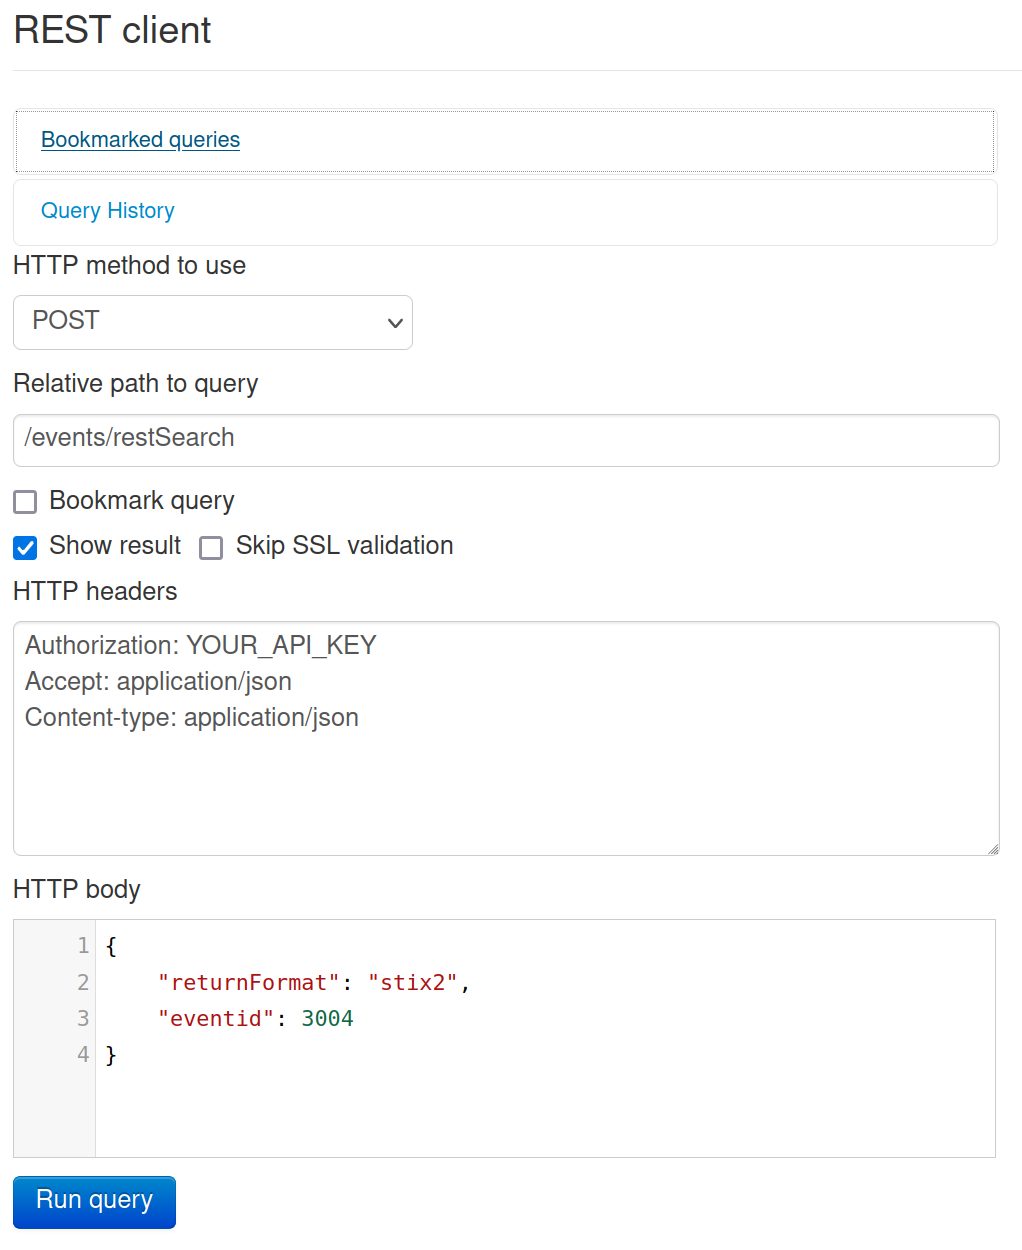
\includegraphics[scale=0.19]{images/simple_rest_query.png}
\end{frame}

\begin{frame}
    \frametitle{STIX conversion usage in MISP}
    \centering
    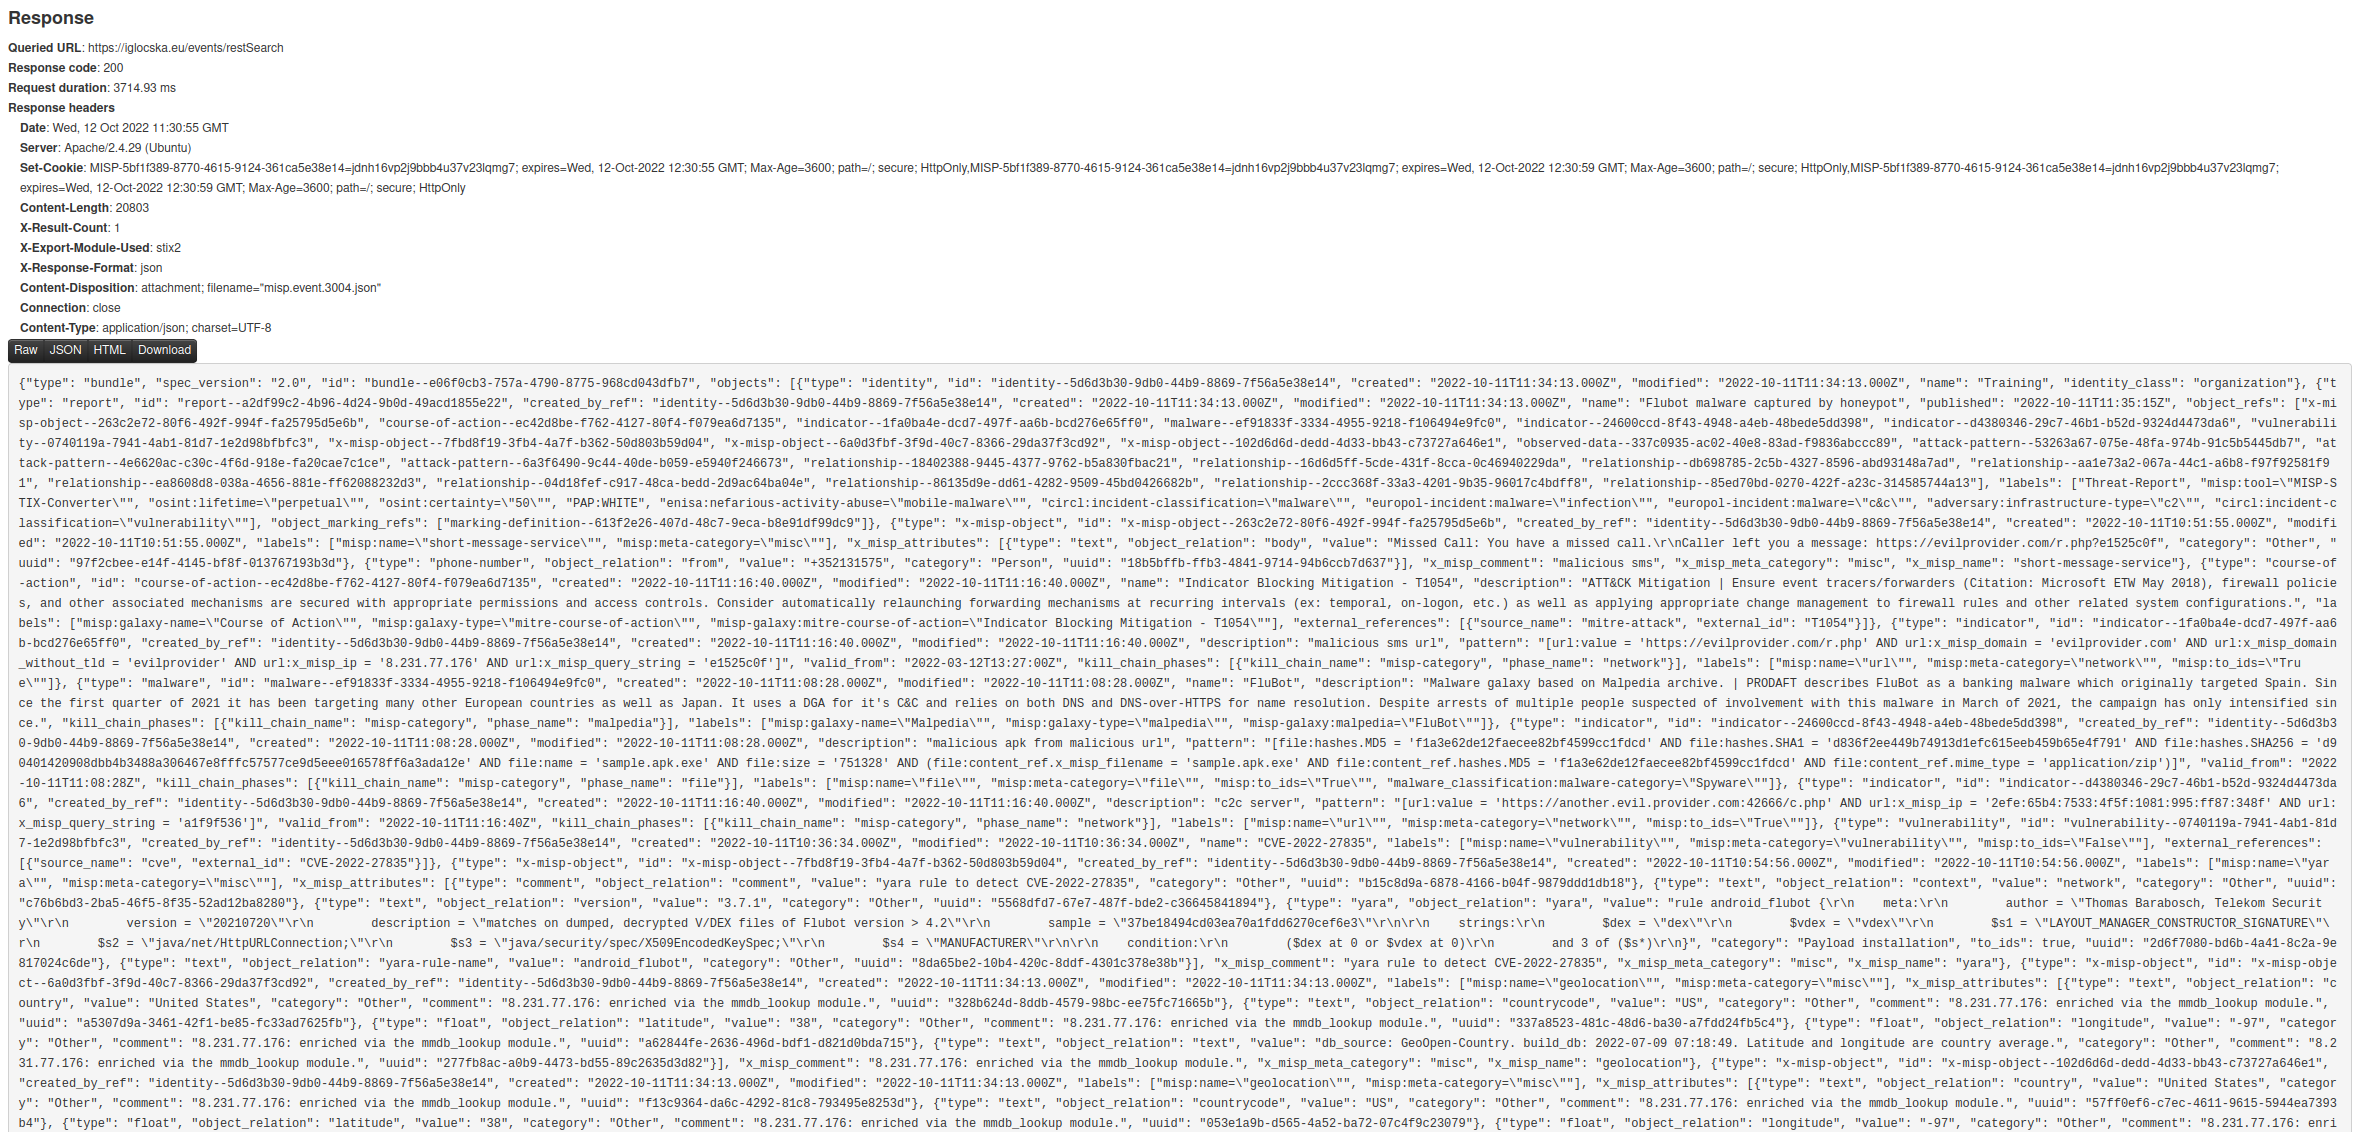
\includegraphics[scale=0.2]{images/simple_rest_results.png}
\end{frame}

\begin{frame}
    \frametitle{STIX conversion usage in MISP}
    \centering
    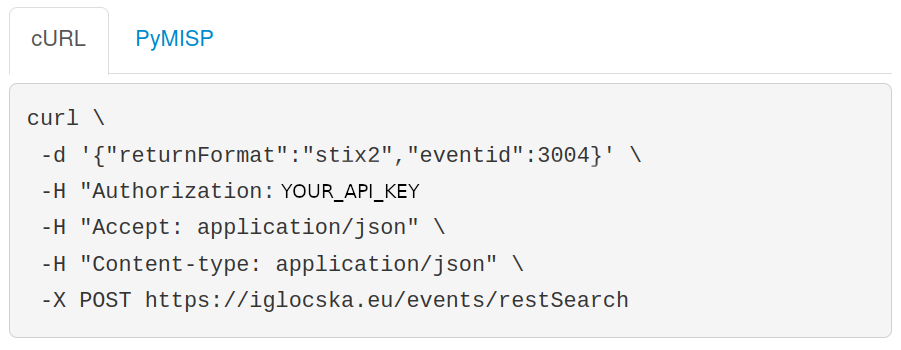
\includegraphics[scale=0.235]{images/simple_rest_curl.png} \\
    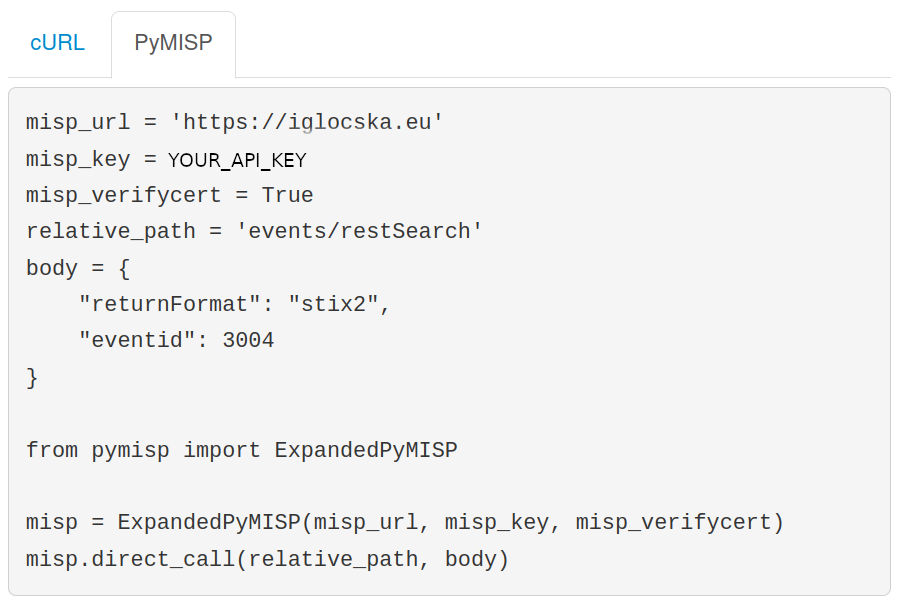
\includegraphics[scale=0.235]{images/simple_rest_pymisp.png}
\end{frame}

\begin{frame}
    \frametitle{Former feature limitations}
    \begin{minipage}{0.45\textwidth}
        \begin{itemize}
            \item {\bf Supported versions}
            \begin{itemize}
                \item 1.1.1 XML (\& JSON)
                \item 2.0
            \end{itemize}
            \item Data type support
        \end{itemize}
    \end{minipage}%
    \begin{minipage}{0.55\textwidth}
        \centering
        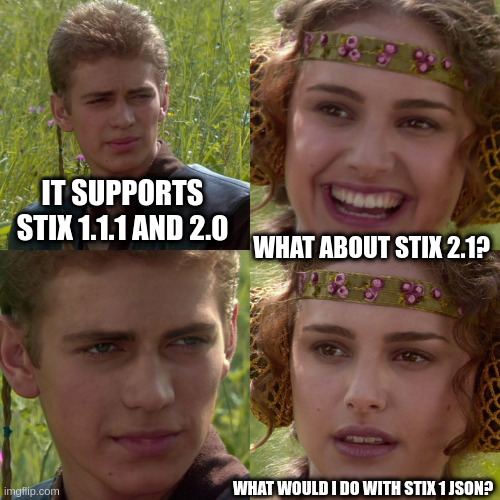
\includegraphics[width=\textwidth]{images/limited_version.jpg}
    \end{minipage}
\end{frame}

\begin{frame}
    \frametitle{Former feature limitations}
    \begin{minipage}{0.5\textwidth}
        \begin{itemize}
            \item Supported versions
            \begin{itemize}
                \item 1.1.1 XML (\& JSON)
                \item 2.0
            \end{itemize}
            \item {\bf Data type support}
        \end{itemize}
    \end{minipage}%
    \begin{minipage}{0.5\textwidth}
        \centering
        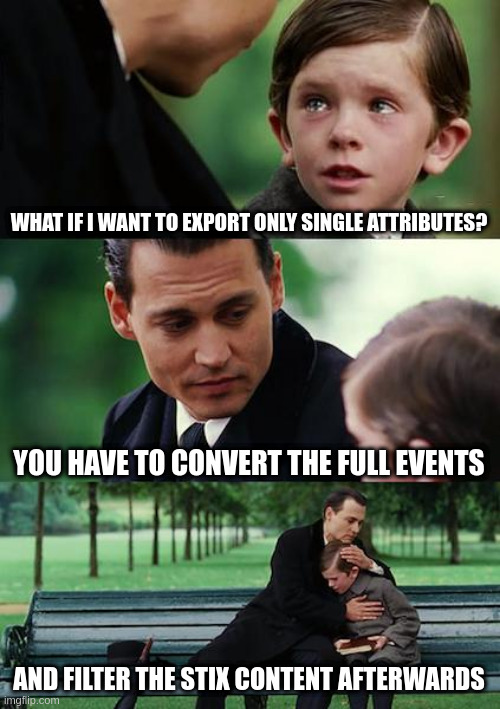
\includegraphics[width=\textwidth]{images/limited_data_type.jpg}
    \end{minipage}
\end{frame}

\begin{frame}
    \frametitle{Former practical \& Organisational limitations}
    \begin{itemize}
        \item Export and import features only available via MISP
        \begin{itemize}
            \item Need an automation key (and/or to deal with the UI)
        \end{itemize}
        \item []
        \item {\bf Github}: STIX issues lost within the MISP core issues
        \pause
        \vspace{4em}
        \begin{center}
            
\includegraphics[scale=0.4]{images/issues.png}
        \end{center}
    \end{itemize}
\end{frame}

\begin{frame}
    \frametitle{The solution}
    \begin{center}
        
\includegraphics[scale=0.3]{images/solution.png}
    \end{center}
\end{frame}

\begin{frame}
    \frametitle{Key features}
    \begin{itemize}
        \item Support all the STIX versions
        \begin{itemize}
            \item {\bf STIX 2.1 Support}
            \item 1.1.1, 1.2, 2.0 Support enhanced
        \end{itemize}
        \item Various MISP data collection supported
        \item[]
        \item {\bf Mapping documentation}
    \end{itemize}
\end{frame}

\begin{frame}
    \frametitle{Handling the conversion with a python library}
    \begin{itemize}
        \item Used in MISP built-in export modules
        \item []
        \item Enable a {\bf stand-alone} use of the python code\footnote{i.e command line}
        \begin{itemize}
            \item Pass filenames \& get the converted content written in 1 or more result file(s)
        \end{itemize}
        \item Possible integration within python code
        \begin{itemize}
            \item Give it a list of filenames
            \item MISP standard format <-> STIX
            \begin{itemize}
                \item JSON or PyMISP
            \end{itemize}
        \end{itemize}
    \end{itemize}
\end{frame}

\begin{frame}
    \frametitle{Library usage - Command line}
    \centering
    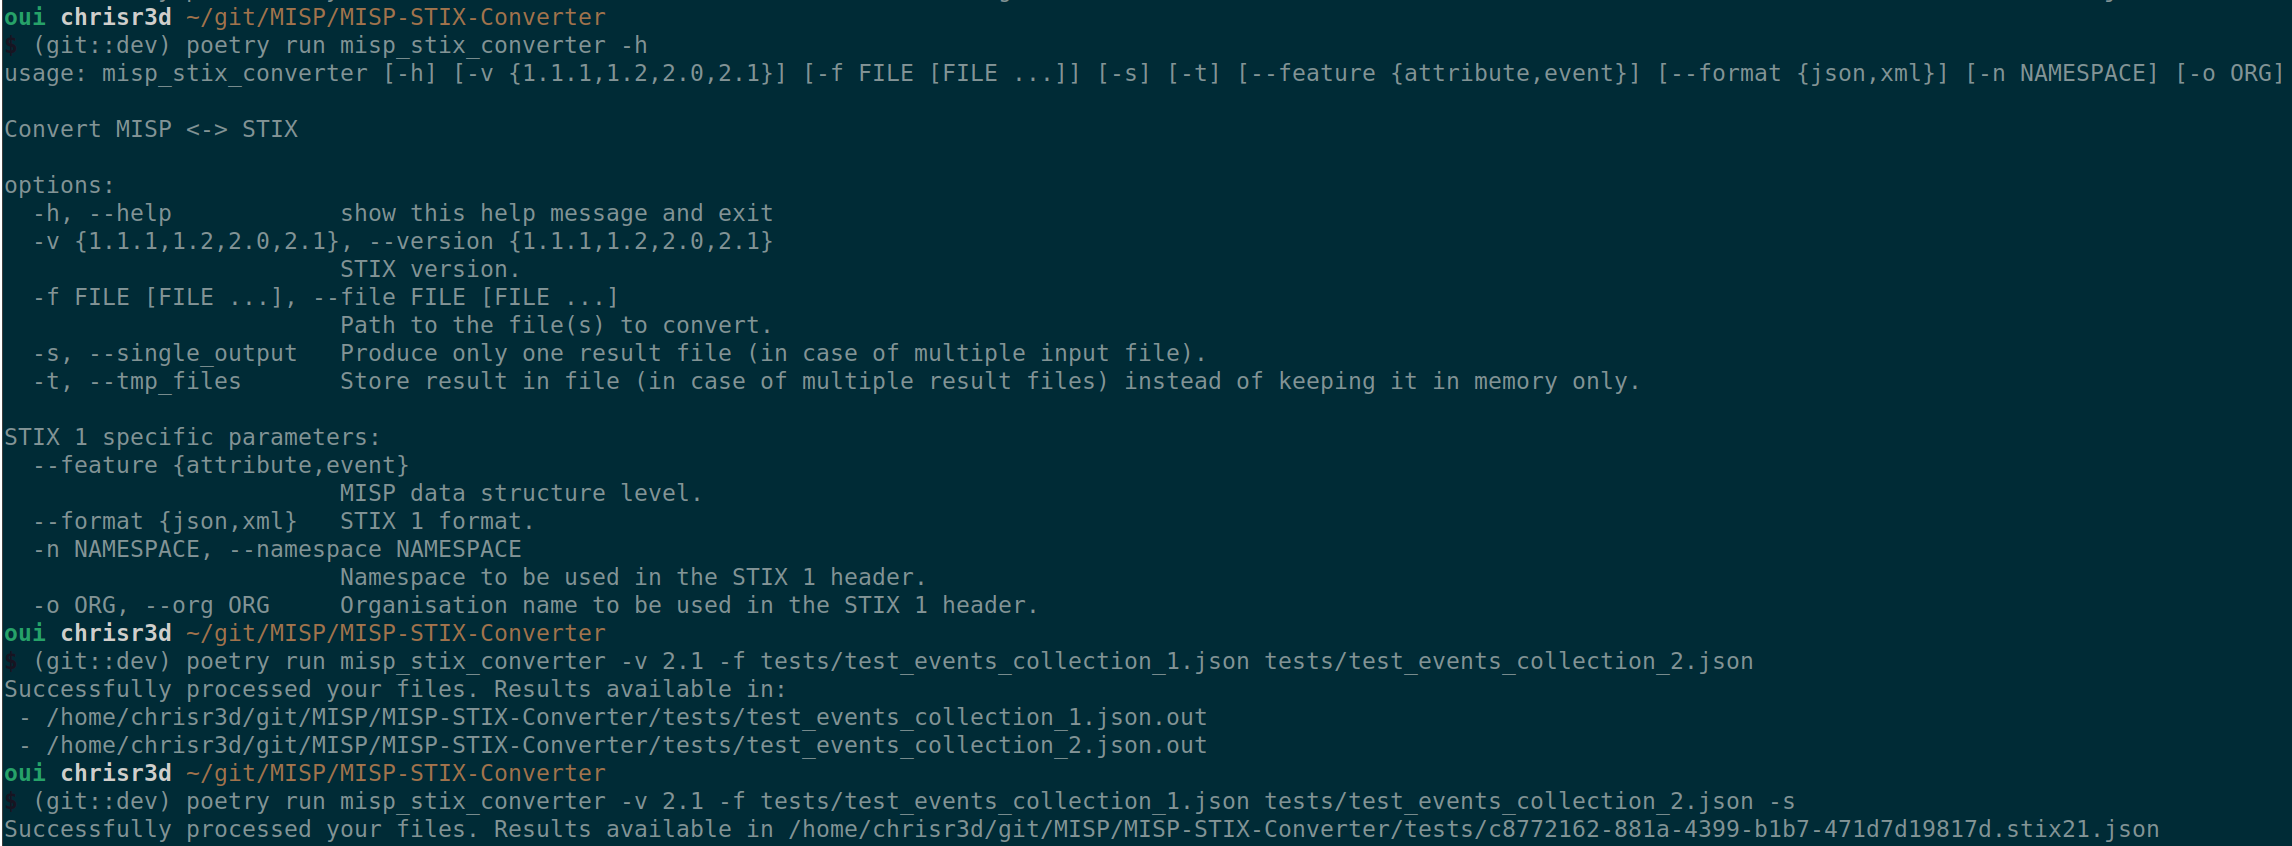
\includegraphics[scale=0.145]{images/stand_alone_usage.png}
\end{frame}

\begin{frame}
    \frametitle{Library usage - Python integration}
    \centering
    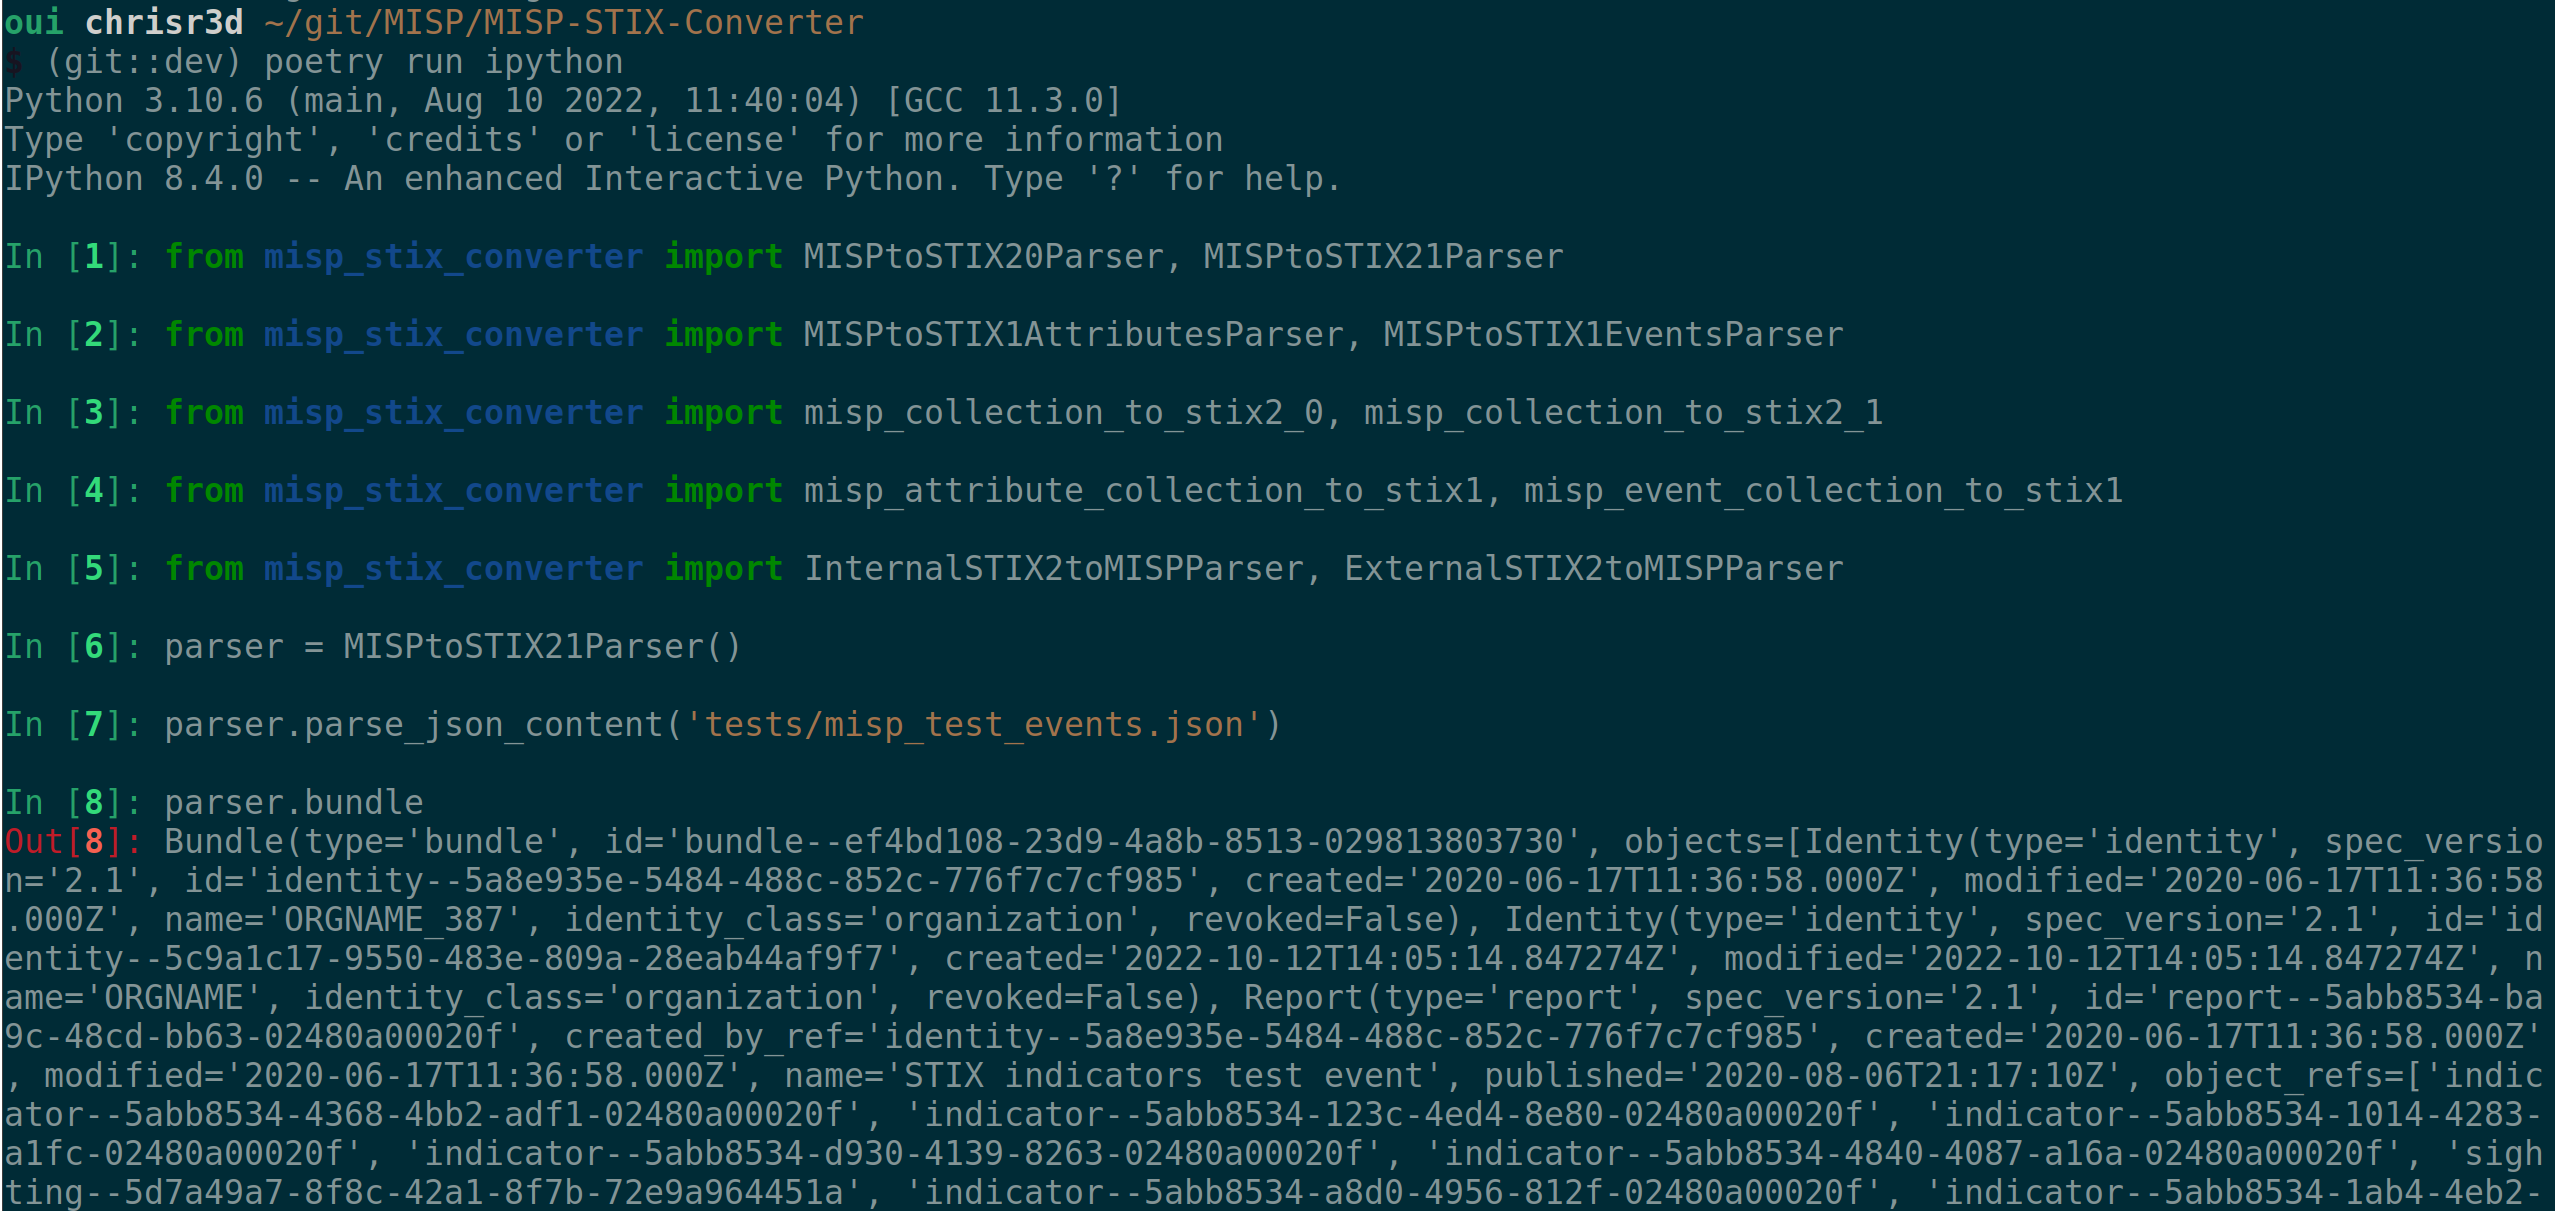
\includegraphics[scale=0.12]{images/python_usage.png}
\end{frame}

\begin{frame}
    \frametitle{Mapping documentation}
    \begin{itemize}
        \item Mapping overview
        \begin{itemize}
            \item Quick overview on how MISP data structures are mapped with STIX objects
        \end{itemize}
        \item []
        \item Detailed mapping
        \begin{itemize}
            \item Extended explanation on how each granular data is mapped with STIX objects fields
        \end{itemize}
    \end{itemize}
\end{frame}

\begin{frame}
    \frametitle{Mapping explained}
    \centering
    
\includegraphics[scale=0.45]{images/demo1.jpg}
\end{frame}

\begin{frame}
    \frametitle{Work in Progress \& Continuous development}
    \begin{itemize}
        \item {\bf STIX 2 -> MISP import feature}
        \item []
        \item Current mapping improvement
        \begin{itemize}
            \item Support for Custom Galaxy clusters
            \item Better support of existing STIX objects libraries\footnote{e.g: \url{https://github.com/mitre/cti}}
            \item Support custom STIX format\footnote{e.g: ACS custom markings}
        \end{itemize}
    \end{itemize}
    \pause
    \begin{minipage}{0.5\textwidth}
        \begin{itemize}
            \item {\bf TAXII integration}
        \end{itemize}
    \end{minipage}%
    \begin{minipage}{0.5\textwidth}
        
\includegraphics[scale=0.2]{images/surprise.jpg}
    \end{minipage}
\end{frame}

\begin{frame}
    \frametitle{What comes next?}
    \begin{itemize}
        \item Extend the export feature to any kind of data collection
        \item []
        \item Add notes on any data structure
        \item Sightings on context layers
        \item []
        \item Port the STIX 1 -> MISP import feature
    \end{itemize}
\end{frame}

\begin{frame}
    \frametitle{Handling different STIX content creation designs}
    \begin{minipage}{0.6\textwidth}
        \begin{itemize}
            \item Impossible to control the content created by external parties
            \item We want to keep UUIDs
            \pause
            \item []
            \item Facing UUIDs validation issues
            \begin{itemize}
                \item Loading error
            \end{itemize}
        \end{itemize}
    \end{minipage}%
    \begin{minipage}{0.4\textwidth}
        
\includegraphics[scale=0.25]{images/two_buttons_dilemna.jpg}
    \end{minipage}
\end{frame}

\begin{frame}
    \frametitle{An easy fix: a STIX 2 python library fork\footnote{\url{https://github.com/MISP/cti-python-stix2} \& \url{https://pypi.org/project/misp-lib-stix2/}}}
    \begin{minipage}{0.62\textwidth}
        \begin{itemize}
            \item No change on the content validation
            \begin{itemize}
                \item Differs only on the UUIDs validation process
            \end{itemize}
            \item MISP has now the same UUIDs requirements
            \begin{itemize}
                \item We keep a reference to the initial UUID
                \item A UUID v5 is generated
            \end{itemize}
        \end{itemize}
    \end{minipage}%
    \begin{minipage}{0.38\textwidth}
        
\includegraphics[scale=0.25]{images/two_buttons_solution.jpg}
    \end{minipage}
\end{frame}

\begin{frame}
    \frametitle{Minding the gap between formats}
    \begin{itemize}
        \item From a sharing platform to an threat intelligence exchange format
        \begin{itemize}
            \item Custom STIX objects
            \item Custom fields in existing objects
            \item STIX extensions
        \end{itemize}
        \item Handling the infinite possibilities of a patterning language
        \begin{itemize}
            \item Importing STIX 2 patterns in separate MISP objects
        \end{itemize}
    \end{itemize}
    \pause
    \vspace{1em}
    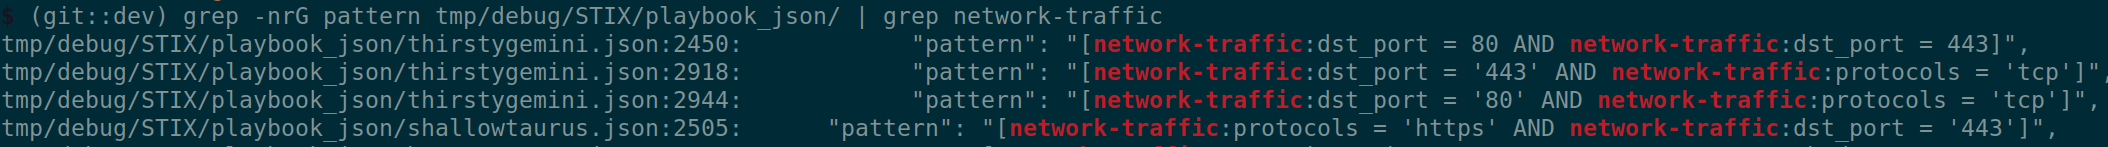
\includegraphics[scale=0.15]{images/patterns.png}
\end{frame}

\begin{frame}
    \frametitle{Mapping challenges}
    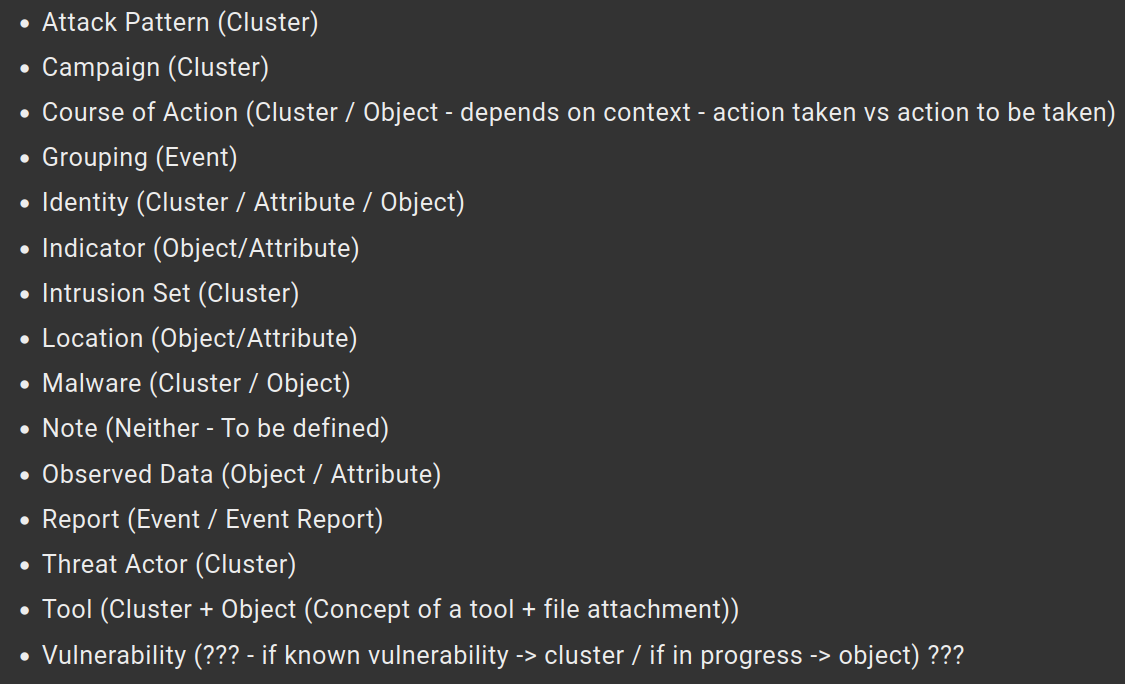
\includegraphics[scale=0.285]{images/challenges.png}
\end{frame}

\begin{frame}
    \frametitle{Evolution perspectives}
    \begin{center}
        
\includegraphics[scale=0.1]{images/oasis.png}
    \end{center}
    \vspace{1em}
    \begin{itemize}
        \item Members of the Oasis CTI TC
        \begin{itemize}
            \item Our involvement
            \begin{itemize}
                \item Participating to the development process
            \end{itemize}
            \item []
            \item Our proposal: Go for the open source way
            \begin{itemize}
                \item Make the contribution process more accessible \\
                => Bring more contributers / contributions
                \item Easier access to the resources \\
                => More visibility
            \end{itemize}
        \end{itemize}
    \end{itemize}
\end{frame}

\begin{frame}
    \frametitle{How to report bugs/issues}
    \begin{itemize}
        \item Github issues
        \begin{itemize}
            \item {\bf \url{https://github.com/MISP/misp-stix/issues}}
            \item \url{https://github.com/MISP/MISP/issues}
        \end{itemize}
        \item []
        \item Please provide details
        \begin{itemize}
            \item How did the issue happen
            \item {\bf Recommendation}: provide samples
        \end{itemize}
        \item[]
        \item Any feedback welcome
    \end{itemize}
\end{frame}

\begin{frame}
    \frametitle{Useful links}
    \begin{itemize}
        \item \url{https://github.com/MISP/misp-stix}
        \item \url{https://github.com/MISP/misp-stix/tree/main/documentation}
        \item []
        \item \url{https://github.com/MISP}
        \item \url{https://www.misp-project.org/}
        \item \url{https://twitter.com/MISPProject}
        \item \url{https://twitter.com/chrisred_68}
    \end{itemize}
\end{frame}

\begin{frame}
    \frametitle{Demo time}
    \centering
    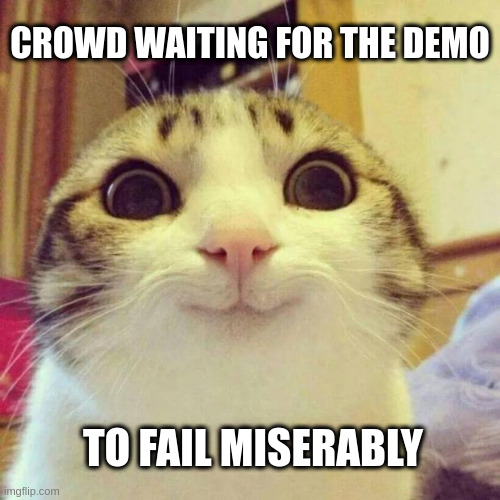
\includegraphics[scale=0.45]{images/demo2.jpg}
\end{frame}
